\begin{figure}[htbp]
	\centering
	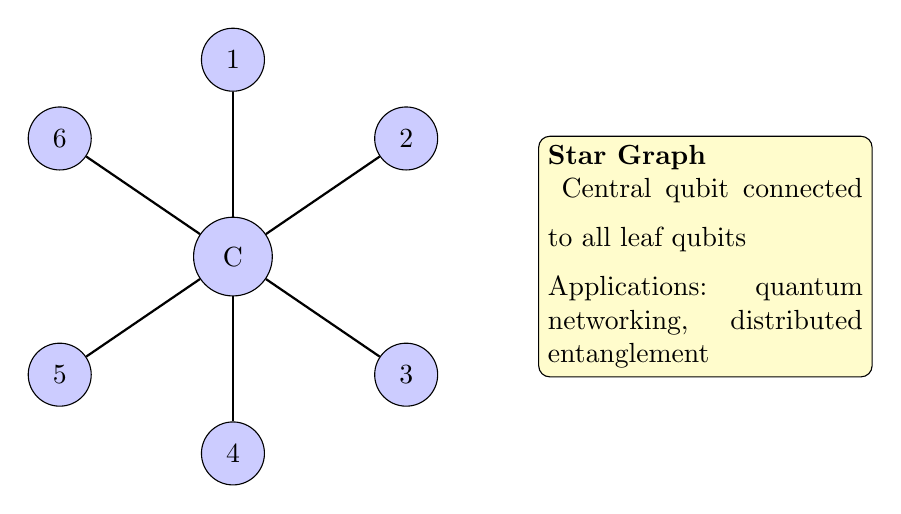
\begin{tikzpicture}
		\node[draw, circle, fill=blue!20, minimum size=1cm] (center) at (0,0) {C};
		\node[draw, circle, fill=blue!20, minimum size=0.8cm] (1) at (0,2.5) {1};
		\node[draw, circle, fill=blue!20, minimum size=0.8cm] (2) at (2.2,1.5) {2};
		\node[draw, circle, fill=blue!20, minimum size=0.8cm] (3) at (2.2,-1.5) {3};
		\node[draw, circle, fill=blue!20, minimum size=0.8cm] (4) at (0,-2.5) {4};
		\node[draw, circle, fill=blue!20, minimum size=0.8cm] (5) at (-2.2,-1.5) {5};
		\node[draw, circle, fill=blue!20, minimum size=0.8cm] (6) at (-2.2,1.5) {6};

		\draw[thick] (center) -- (1);
		\draw[thick] (center) -- (2);
		\draw[thick] (center) -- (3);
		\draw[thick] (center) -- (4);
		\draw[thick] (center) -- (5);
		\draw[thick] (center) -- (6);

		\node[draw, rounded corners, fill=yellow!20] at (6,0) {
			\begin{minipage}{4cm}
				\textbf{Star Graph}\\
				\vspace{0.2cm}
				Central qubit connected to all leaf qubits\\[0.2cm]
				Applications: quantum networking, distributed entanglement
			\end{minipage}
		};
	\end{tikzpicture}
	\caption{Star graph configuration. The central qubit (C) is connected to all leaf qubits. Star graph states are highly symmetric and useful for quantum networking protocols where entanglement needs to be distributed from a central node.}
	\label{fig:star-graph}
\end{figure}
